\documentclass[12pt]{article}

\usepackage{amsmath, mathtools}
\usepackage{amsfonts}
\usepackage{amssymb}
\usepackage{graphicx}
\usepackage{colortbl}
\usepackage{xr}
\usepackage{hyperref}
\usepackage{longtable}
\usepackage{xfrac}
\usepackage{tabularx}
\usepackage{float}
\usepackage{siunitx}
\usepackage{booktabs}
\usepackage{caption}
\usepackage{pdflscape}
\usepackage{afterpage}

\usepackage[round]{natbib}

%\usepackage{refcheck}

\hypersetup{
    bookmarks=true,         % show bookmarks bar?
      colorlinks=true,       % false: boxed links; true: colored links
    linkcolor=red,          % color of internal links (change box color with linkbordercolor)
    citecolor=green,        % color of links to bibliography
    filecolor=magenta,      % color of file links
    urlcolor=cyan           % color of external links
}

%% Comments

\usepackage{color}

\newif\ifcomments\commentstrue

\ifcomments
\newcommand{\authornote}[3]{\textcolor{#1}{[#3 ---#2]}}
\newcommand{\todo}[1]{\textcolor{red}{[TODO: #1]}}
\else
\newcommand{\authornote}[3]{}
\newcommand{\todo}[1]{}
\fi

\newcommand{\wss}[1]{\authornote{blue}{SS}{#1}}
\newcommand{\an}[1]{\authornote{magenta}{Author}{#1}}


% For easy change of table widths
\newcommand{\colZwidth}{1.0\textwidth}
\newcommand{\colAwidth}{0.13\textwidth}
\newcommand{\colBwidth}{0.82\textwidth}
\newcommand{\colCwidth}{0.1\textwidth}
\newcommand{\colDwidth}{0.05\textwidth}
\newcommand{\colEwidth}{0.8\textwidth}
\newcommand{\colFwidth}{0.17\textwidth}
\newcommand{\colGwidth}{0.5\textwidth}
\newcommand{\colHwidth}{0.28\textwidth}

% Used so that cross-references have a meaningful prefix
\newcounter{defnum} %Definition Number
\newcommand{\dthedefnum}{GD\thedefnum}
\newcommand{\dref}[1]{GD\ref{#1}}
\newcounter{datadefnum} %Datadefinition Number
\newcommand{\ddthedatadefnum}{DD\thedatadefnum}
\newcommand{\ddref}[1]{DD\ref{#1}}
\newcounter{theorynum} %Theory Number
\newcommand{\tthetheorynum}{T\thetheorynum}
\newcommand{\tref}[1]{T\ref{#1}}
\newcounter{tablenum} %Table Number
\newcommand{\tbthetablenum}{T\thetablenum}
\newcommand{\tbref}[1]{TB\ref{#1}}
\newcounter{assumpnum} %Assumption Number
\newcommand{\atheassumpnum}{P\theassumpnum}
\newcommand{\aref}[1]{A\ref{#1}}
\newcounter{goalnum} %Goal Number
\newcommand{\gthegoalnum}{P\thegoalnum}
\newcommand{\gsref}[1]{GS\ref{#1}}
\newcounter{instnum} %Instance Number
\newcommand{\itheinstnum}{IM\theinstnum}
\newcommand{\iref}[1]{IM\ref{#1}}
\newcounter{reqnum} %Requirement Number
\newcommand{\rthereqnum}{P\thereqnum}
\newcommand{\rref}[1]{R\ref{#1}}
\newcounter{lcnum} %Likely change number
\newcommand{\lthelcnum}{LC\thelcnum}
\newcommand{\lcref}[1]{LC\ref{#1}}

\newcommand{\progname}{Stock Prediction System} % PUT YOUR PROGRAM NAME HERE

\usepackage{fullpage}

\begin{document}

\title{Stock Prediction System} 
\author{Renjie Zhang}
\date{\today}
	
\maketitle

~\newpage

\pagenumbering{roman}

\section{Revision History}

\begin{tabularx}{\textwidth}{p{3cm}p{2cm}X}
\toprule {\bf Date} & {\bf Version} & {\bf Notes}\\
\midrule
2017-09-25  & 1.0 & create\\
2017-10-04  & 1.1 & update\\
\bottomrule
\end{tabularx}

~\newpage

\section{Reference Material}

This section records information for easy reference.

\subsection{Table of Units}

~\newline

\renewcommand{\arraystretch}{1.2}
%\begin{table}[ht]
  \noindent \begin{tabular}{l l l} 
    \toprule		
    \textbf{symbol} & \textbf{unit} & \textbf{SI}\\
    \midrule 
    \si{\$} & currency & dollar\\

    \bottomrule
  \end{tabular}
  %	\caption{Provide a caption}
%\end{table}


\subsection{Table of Symbols}


\renewcommand{\arraystretch}{1.2}
%\noindent \begin{tabularx}{1.0\textwidth}{l l X}
\noindent \begin{longtable*}{l l p{12cm}} \toprule
\textbf{symbol} & \textbf{unit} & \textbf{description}\\
\midrule 
$K$ & \si[per-mode=symbol] {} & The Kernel use to solve the non-linear classification\\
$y$ & \si[per-mode=symbol] {integer} & can be 1 or -1, use to represent the result. 1 means increase, -1 is decrease.\\
$\sigma$ & \si[per-mode=symbol] {percentage} & Stock Price Volality (see 5.2.4 for detail)\\ 
$C$ & \si[per-mode=symbol] {price} & stock daily price\\ 
\bottomrule
\end{longtable*}


\subsection{Abbreviations and Acronyms}

\renewcommand{\arraystretch}{1.2}
\begin{tabular}{l l} 
  \toprule		
  \textbf{symbol} & \textbf{description}\\
  \midrule 
  A & Assumption\\
  DD & Data Definition\\
  GD & General Definition\\
  GS & Goal Statement\\
  IM & Instance Model\\
  LC & Likely Change\\
  PS & Physical System Description\\
  R & Requirement\\
  SRS & Software Requirements Specification\\
  \progname{} & {Stock Prediction System}\\
  T & Theoretical Model\\
  SVM & Support Vector Machinel\\
  \bottomrule
\end{tabular}\\


\newpage

\tableofcontents

~\newpage

\pagenumbering{arabic}

\section{Introduction}
Stock price prediction is a popular and challenging topic nowadays.There were serveral prediction models such as linear statistical time series models. With the development of Big Data and Machine learning, the prediction technology may have a significant improvement. 
This project will introduce a stock prediction system is used to analyze the future trend of stocks. The prediction was provided by machine learning algorithms based on the historical data. 
The system will be run on a big data platform (Spark), in order to obtain the more accurate results. In this case, we need to setup a distributed system to support Spark.

\subsection{Purpose of Document}
The purpose of this document is to explain how to implement a machine learning system for stock price prediction.   With different algorithms and dataset, the system can be used for both short term and long term predictions.
In this case, we will use Support Vector Machine to predict the future trend of stocks based on the daily historical data. 
\subsection{Scope of Requirements} 
The purpose of this software is to give the user a reference by calculating the possibility of the future price change. For example, it may go up with a chance of xx percent and go down with a chance of xx percent. 
\subsection{Characteristics of Intended Reader} 
Reader are not required to have any specific  background knowledge. However, it is very helpful to have some basic knowledge of big data, machine learning, especially Support Vector Machine.
\subsection{Organization of Document}
This document will cover the configuration of the Spark distributed system for big data, the workflow of the program and the explaination of SVM algorithm.
\section{General System Description}

The project have an interface to let the user choose the company, but on the demo there will be only one company to display. It loads the historical data provided by the user and caculate the future trend. A plot graph will be displayed  as well. There will be two results come out, one is the possibility of increase and the other is of decrease.

\subsection{System Context}

\begin{itemize}
\item User Responsibilities:
\begin{itemize}
\item Prepare the historical data file
\item Decide the date time range of the historical period
\item Update the historical data set
\end{itemize}
\item \progname{} Responsibilities:
\begin{itemize}
\item Load data  from files and display errors when the loading failes
\item Display the plot of the stock
\item Predict the future trent based on the historical data with the possibilities
\end{itemize}
\end{itemize}

\subsection{User Characteristics} \label{SecUserCharacteristics}

The end user of \progname{} should have some basic knowledge of machine learning algorithm (Support Vector Machine).

\subsection{System Constraints}
The system supports multiple operating systems. However, since it is running on Spark, it is more stable with Linux/Ubuntu. The program needs a distributed systtem consist of at lease three computers, one will be the driver of Spark, the others will be the workers.

\section{Specific System Description}

This system is used to predict the future trend of stocks based on the historical data from Yahoo Finance using Support Vector Machine algorithm. The data from other resource is acceabled if they fit the format. The programming language will be Python.

\subsection{Problem Description} \label{Sec_pd}

Stock Prediction is a very important topic in financial industry. It is  complicated because the stock price was affected by too many factors. One of the common prediction technology is to train and test the historical data using machin learning.
\progname{} is a tool to predict stocks based on machine learning and big data. It implements SVM classifier to train and test the historical data.  With the development of Big Data and Machine learning, it is possible to obtain an more accurate prediction result. 
To delivery a more accurate result, a large scale of data is needed. In this case it is nessary to run the program on a distributed system platform such as Spark to accerate the caculation speed.


\subsubsection{Terminology and  Definitions}

This subsection provides a list of terms that are used in the subsequent
sections and their meaning, with the purpose of reducing ambiguity and making it
easier to correctly understand the requirements:

\begin{itemize}

\item Support Vector Machine  :
A supervised learning model with associated learning algorithms that analyze data used for classification and regression analysis.
\item Spark :
A big data platform that save and retrive data from different machines in a format called RDD(Resilient Distributed Datasets). It provides a set of machine learning libraries and support different types of programming lanauges. 
\item RDD :
Resilient Distributed Datasets (RDD) is a fundamental data structure of Spark. It is an immutable distributed collection of objects. Each dataset in RDD is divided into logical partitions, which may be computed on different nodes of the cluster.
\item Distributed System :
A distributed system is a model in which components located on networked computers communicate and coordinate their actions by passing messages. It combines a set of computers to work on a single task as one machine.
\item Training and Testing :
A training set is a set of data used to discover potentially predictive relationships. A test set is a set of data used to assess the strength and utility of a predictive relationship. Test and training sets are used in intelligent systems, machine learning, genetic programming and statistics.

\end{itemize}

\subsubsection{Physical System Description}

The physical system of \progname{}, is a distributed system consists by a driver and 2-3 works as shown in Figure~?,
includes the following elements:

\begin{itemize}

\item Driver (Master) : 
The drive is the machine that send requests to the works and receive the response from, it some times called Master. Data will be converted into RDD format and equaly assigned to each work. Drive itself does not do the actual works and there is only on drive in the distributed system.

\item Worker (Slave): 
The workers are the machines which do the actual jobs and they are called slaves as well. They receive data from drive using RDD and return an RDD back to drive after certain processes.  For each distributed system, there are at least 2 workers, otherwise it will work as a single node computers. Each worker has a copy of the program.  


\end{itemize}


\begin{figure}[h!]
\begin{center}
%\rotatebox{-90}
{
  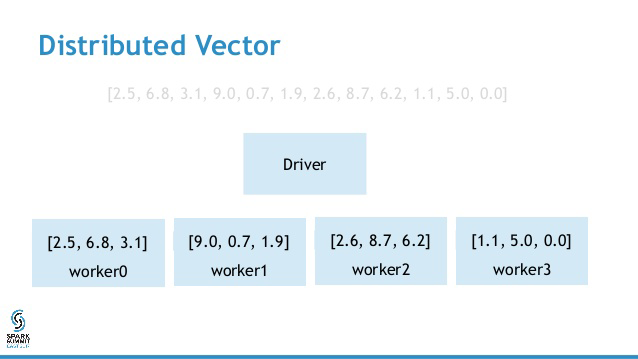
\includegraphics[width=0.5\textwidth]{sparkrdd.png}
 }
 \caption{\label{Spark}}
 \end{center}
 \end{figure}

\subsubsection{Goal Statements}

\begin{itemize}

\item Predicture Result\refstepcounter{goalnum}\thegoalnum \label{G_meaningfulLabel}: A result of the future stock price with its probability.

\end{itemize}

\subsection{Solution Characteristics Specification}

The instance models that govern \progname{} are presented in
Subsection~\ref{sec_instance}.  The information to understand the meaning of the
instance models and their derivation is also presented, so that the instance
models can be verified.

\subsubsection{Assumptions}

This section simplifies the original problem and helps in developing the
theoretical model by filling in the missing information for the physical
system. The numbers given in the square brackets refer to the theoretical model
[T], general definition [GD], data definition [DD], instance model [IM], or
likely change [LC], in which the respective assumption is used.

\begin{itemize}

\item[A\refstepcounter{assumpnum}\theassumpnum \label{Ass1}:]
Efficient Markets Hypothesis holds true. It posits that stock prices already reflected all available information and are there fore unpredictable. 

\item[A\refstepcounter{assumpnum}\theassumpnum \label{Ass2}:]
Independent identically distributed. A sequence or other collection of random variables is independent and identically distributed (i.i.d. or iid or IID) if each random variable has the same probability distribution as the others and all are mutually independent.

\item[A\refstepcounter{assumpnum}\theassumpnum \label{Ass3}:]
All companies are active on NASDAQ during the period of 2003-2012.

\item[A\refstepcounter{assumpnum}\theassumpnum \label{Ass4}:]
The historical data is daily.

\end{itemize}

\subsubsection{Theoretical Models}\label{sec_theoretical}

This section focuses on the general equations and laws that \progname{} is based
on. 

~\newline
%T1
\noindent
\begin{minipage}{\textwidth}
\renewcommand*{\arraystretch}{1.5}
\begin{tabular}{| p{\colAwidth} | p{\colBwidth}|}
  \hline
  \rowcolor[gray]{0.9}
  Number& T\refstepcounter{theorynum}\thetheorynum \label{T_COE}\\
  \hline
  Label&\bf Support Vector Machine\\
  \hline
  Equation&  $y=\beta _0+\sum {a_iy_iK(x(i),x)}$\\
  \hline
  Description & 
	     
The above equation gives a linear classification in a higher dimensional space and linearly classify in that space.   $x$ is an n-dimensional feature vector $x=(X_1,.....X_n)$. $y\in \left \{ 1,-1 \right \}$ is the label, in a range of 1 and -1.
This SVM replaces the inner product with a more general kernel function K which allows the input to be mapped to higher-dimensions. In this case, RBF Kernel is used for price forcasting.    \\
  \hline
  Source &
           \url{https://www.cs.princeton.edu/sites/default/files/uploads/saahil_madge.pdf}\\
  % The above web link should be replaced with a proper citation to a publication
  \hline
  Ref.\ By & \ddref{StockPV} \\
  \hline
\end{tabular}
\end{minipage}\\

~\newline

~\newline
%T2
\noindent
\begin{minipage}{\textwidth}
\renewcommand*{\arraystretch}{1.5}
\begin{tabular}{| p{\colAwidth} | p{\colBwidth}|}
  \hline
  \rowcolor[gray]{0.9}
  Number& T\refstepcounter{theorynum}\thetheorynum \label{T_SHE}\\
  \hline
  Label&\bf Specific Kernel Function\\
  \hline
 Equation&  $k\left (X_i,X_k\right )=\exp \left ( -\frac1{\delta^2}\sum_{n}^{j=1}(X_{ij}-X_{kj})^2 \right )$ \\
  \hline
  Description & 
	     
Where  $delta$ is known as the bandwidth of the kernel function  \\
  \hline
  Source &
           \url{https://www.cs.princeton.edu/sites/default/files/uploads/saahil_madge.pdf}\\
  % The above web link should be replaced with a proper citation to a publication
  \hline
  Ref.\ By & \ddref{StockPV} \\
  \hline
\end{tabular}
\end{minipage}\\

~\newline

\subsubsection{General Definitions}\label{sec_gendef}

There is no General Definitions applied on this project.

~\newline



\subsubsection{Data Definitions}\label{sec_datadef}

This section collects and defines all the data needed to build the instance
models. The dimension of each quantity is also given. 

%DD1
~\newline

\noindent
\begin{minipage}{\textwidth}
\renewcommand*{\arraystretch}{1.5}
\begin{tabular}{| p{\colAwidth} | p{\colBwidth}|}
\hline
\rowcolor[gray]{0.9}
Number& DD\refstepcounter{datadefnum}\thedatadefnum \label{StockPV}\\
\hline
Label& \bf Stock Price Volatility\\
\hline
Symbol &$\sigma_s$\\
\hline
% Units& $Mt^{-3}$\\
% \hline
  SI Units & \% percentage\\
  \hline
  Equation&$\frac{\sum_{i=t-n+1}^{t} \frac{C_i-C_{i-1}}{C{i-1}}}{n}$  

\\
  \hline
  Description & 
         Stock price is an average over the past $n$ days of percent change in the given stock’s price per day  \\
  \hline
  Sources&
   \url{https://www.cs.princeton.edu/sites/default/files/uploads/saahil_madge.pdf}\\
  \hline
  Ref.\ By & \iref{adjClose}\\
  \hline
\end{tabular}
\end{minipage}\\


%DD2
~\newline

\noindent
\begin{minipage}{\textwidth}
\renewcommand*{\arraystretch}{1.5}
\begin{tabular}{| p{\colAwidth} | p{\colBwidth}|}
\hline
\rowcolor[gray]{0.9}
Number& DD\refstepcounter{datadefnum}\thedatadefnum \label{StockM}\\
\hline
Label& \bf Stock Momentum\\
\hline
Symbol & NA\\
\hline
% Units& $Mt^{-3}$\\
% \hline
  SI Units & \$ price\\
  \hline
  Equation& $\frac{\sum_{i=t-n+1}^{t} y}{n}$  \\
  \hline
  Description & 
       This is an average of the given stock’s momentum over the past $n$ days. Each day is labeled 1 if closing price that day is higher than the day before, and −1 if the price is lower than the day before  \\
  \hline
  Sources&
   \url{https://www.cs.princeton.edu/sites/default/files/uploads/saahil_madge.pdf}\\
  \hline
  Ref.\ By & \iref{adjClose}\\
  \hline
\end{tabular}
\end{minipage}\\


%DD3
~\newline

\noindent
\begin{minipage}{\textwidth}
\renewcommand*{\arraystretch}{1.5}
\begin{tabular}{| p{\colAwidth} | p{\colBwidth}|}
\hline
\rowcolor[gray]{0.9}
Number& DD\refstepcounter{datadefnum}\thedatadefnum \label{IndexV}\\
\hline
Label& \bf Index Volatility\\
\hline
Symbol &$\sigma_i$\\
\hline
% Units& $Mt^{-3}$\\
% \hline
  SI Units & \% percentage\\
  \hline
  Equation&$\frac{\sum_{i=t-n+1}^{t} \frac{I_i-I_{i-1}}{I{i-1}}}{n}$  \\
  \hline
  Description & 
      This is an average over the past $n$ days of percent change in the index's price perday \\
  \hline
  Sources&
   \url{https://www.cs.princeton.edu/sites/default/files/uploads/saahil_madge.pdf}\\
  \hline
  Ref.\ By & \iref{adjClose}\\
  \hline
\end{tabular}
\end{minipage}\\



%DD4
~\newline

\noindent
\begin{minipage}{\textwidth}
\renewcommand*{\arraystretch}{1.5}
\begin{tabular}{| p{\colAwidth} | p{\colBwidth}|}
\hline
\rowcolor[gray]{0.9}
Number& DD\refstepcounter{datadefnum}\thedatadefnum \label{IndexM}\\
\hline
Label& \bf Index Momentum\\
\hline
Symbol & NA\\
\hline
% Units& $Mt^{-3}$\\
% \hline
  SI Units & \$ price\\
  \hline
  Equation& $\frac{\sum_{i=t-n+1}^{t} d}{n}$  \\
  \hline
  Description & 
     This is an average of the index’s momentum over the past n days. Each day is labeled $1$ if closing price that day is higher than the day before, and $−1$ if the price is lower than the day before \\
  \hline
  Sources&
   \url{https://www.cs.princeton.edu/sites/default/files/uploads/saahil_madge.pdf}\\
  \hline
  Ref.\ By & \iref{adjClose}\\
  \hline
\end{tabular}
\end{minipage}\\


\subsubsection{Instance Models} \label{sec_instance}    

This section transforms the problem defined in Section~\ref{Sec_pd} into 
one which is expressed in mathematical terms. It uses concrete symbols defined 
in Section~\ref{sec_datadef} to replace the abstract symbols in the models 
identified in Sections~\ref{sec_theoretical} and~\ref{sec_gendef}.


~\newline


%Instance Model 1

\noindent
\begin{minipage}{\textwidth}
\renewcommand*{\arraystretch}{1.5}
\begin{tabular}{| p{\colAwidth} | p{\colBwidth}|}
  \hline
  \rowcolor[gray]{0.9}
  Number& IM\refstepcounter{instnum}\theinstnum \label{adjClose}\\
  \hline
  Label& \bf Predict future trend by historical data \\
  \hline
  Input& $C_i$ the adjClose, the  Date, the format of the input shown as the figure 2\\
  \hline
  Output& 1 or -1,  the prediction  result \\
  \hline
  Description&
Date is the the date of the trade
~\newline
adjClose stands for the adjusted closing price.  It is a stock's closing price on any give day of trading that has been amended to include any distributions and corporate actions that occurred at any time prior to the next day's open.
~\newline
The result of 1 stands for increase and -1 means decrease.
  \\
  \hline
  Source &
           \url{http://www.investopedia.com/terms/a/adjusted_closing_price.asp}\\
  \hline
  Ref.\ By & \\
  \hline
\end{tabular}
\end{minipage}\\

~\newline
\begin{figure}[h!]
\begin{center}
%\rotatebox{-90}
{
  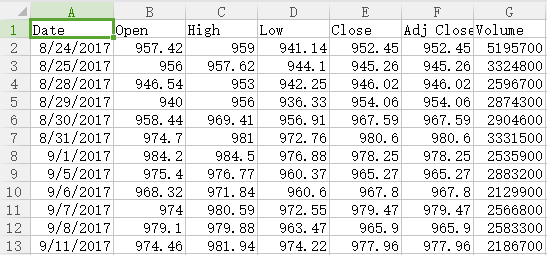
\includegraphics[width=0.5\textwidth]{amazon.png}
 }
 \caption{\label{Input Data}}
 \end{center}
 \end{figure}




\subsubsection{Data Constraints} \label{sec_DataConstraints}    

Tables~\ref{TblInputVar} and \ref{TblOutputVar} show the data constraints on the
input and output variables, respectively.  The column for physical constraints gives
the physical limitations on the range of values that can be taken by the
variable.  The column for software constraints restricts the range of inputs to
reasonable values.  The constraints are conservative, to give the user of the
model the flexibility to experiment with unusual situations.  The column of
typical values is intended to provide a feel for a common scenario.  The
uncertainty column provides an estimate of the confidence with which the
physical quantities can be measured.  This information would be part of the
input if one were performing an uncertainty quantification exercise.

The specification parameters in Table~\ref{TblInputVar} are listed in
Table~\ref{TblSpecParams}.

\begin{table}[!h]
  \caption{Input Variables} \label{TblInputVar}
  \renewcommand{\arraystretch}{1.2}
\noindent \begin{longtable*}{l l l l c} 
  \toprule
  \textbf{Var} & \textbf{Physical Constraints} & \textbf{Software Constraints} &
                             \textbf{Typical Value} & \textbf{Uncertainty}\\
  \midrule 
  $C$ & $C > 0$ & $C > 0$ & \$1000 \si[per-mode=symbol]  & NA
  \\
  \bottomrule
\end{longtable*}
\end{table}

\noindent 
\begin{description}
\item[(*)] 
\end{description}

\begin{table}[!h]
\caption{Specification Parameter Values} \label{TblSpecParams}
\renewcommand{\arraystretch}{1.2}
\noindent \begin{longtable*}{l l} 
  \toprule
 % \textbf{Var} & \textbf{Value} \\
  \midrule 
%  $L_\text{min}$ & 0.1 \si{\metre}\\
  \bottomrule
\end{longtable*}
\end{table}

\begin{table}[!h]
\caption{Output Variables} \label{TblOutputVar}
\renewcommand{\arraystretch}{1.2}
\noindent \begin{longtable*}{l l} 
  \toprule
  \textbf{Var} & \textbf{Physical Constraints} \\
  \midrule 
  $y$ & $1$ or $-1$ 
  \\
  \bottomrule
\end{longtable*}
\end{table}

\subsubsection{Properties of a Correct Solution} \label{sec_CorrectSolution}

\noindent
A correct solution must exhibit. The solution is two results, 1 and -1, each result is with a percentage number.  Any other outputs are incorrect. The result of 1 means the stock is increase, otherwise decreasing.

\section{Requirements}

The required functions are not complex in the system. It basiclly reads a data file and analysis the data then out put a result based on the analysis. 

\subsection{Functional Requirements}

\noindent \begin{itemize}

\item[R\refstepcounter{reqnum}\thereqnum \label{R_Inputs}:] The system must read the input data file provided by the user successfully. This is the first and every other functions rely on it. If the loading has any errors then the whole system will not work. 

\item[R\refstepcounter{reqnum}\thereqnum \label{R_OutputInputs}:] As part of the interface and output, the system needs to generate a graph that explains  the historical data. The graph is a plot consists by the points of stock price and date.  


\item[R\refstepcounter{reqnum}\thereqnum \label{R_Calculate}:] The system needs to calculate the future trend of the stock by training and testing the historical data and finally obtained an acurte result. This is the most important function and it is also the core of the system.

\item[R\refstepcounter{reqnum}\thereqnum \label{R_VerifyOutput}:] The input reading and data calculating must be valid and verified. Invalid data must be skipped and the data type and format must match

\item[R\refstepcounter{reqnum}\thereqnum \label{R_Output}:]  There will be an result about the prediction. The result shows the stock will go up or go down with a probability in a percentage format.
\end{itemize}

\subsection{Nonfunctional Requirements}

The system needs to have a more friendly interface and the layout of the plot graph.

\section{Likely Changes}    

\noindent \begin{itemize}

\item[LC\refstepcounter{lcnum}\thelcnum\label{LC1}:] In short run, we may need intra-day/high frequency data to increase the accuracy.
\item[LC\refstepcounter{lcnum}\thelcnum\label{LC2}:] Try to get more data with longer history and with a larger size of distributed system.
\end{itemize}

\section{Traceability Matrices and Graphs}

The purpose of the traceability matrices is to provide easy references on what
has to be additionally modified if a certain component is changed.  Every time a
component is changed, the items in the column of that component that are marked
with an ``X'' may have to be modified as well.  Table~\ref{Table:trace} shows the
dependencies of theoretical models, general definitions, data definitions, and
instance models with each other. Table~\ref{Table:R_trace} shows the
dependencies of instance models, requirements, and data constraints on each
other. Table~\ref{Table:A_trace} shows the dependencies of theoretical models,
general definitions, data definitions, instance models, and likely changes on
the assumptions.



\afterpage{
\begin{landscape}
\begin{table}[h!]
\centering
\begin{tabular}{|c|c|c|c|c|c|c|c|c|c|c|c|c|c|c|c|c|c|c|c|}
\hline
	& \aref{Ass1}& \aref{Ass2}& \aref{Ass3} & \aref{Ass4}\\
\hline
\tref{T_COE}        & & & & \\ \hline
\tref{T_SHE}         & & & &  \\ \hline
\ddref{StockPV}    & & & &  \\ \hline
\ddref{StockM}     & & & &  \\ \hline
\ddref{IndexV}     & & & &   \\ \hline
\ddref{IndexM}    & & & &  \\ \hline
\iref{adjClose}      &X &X &X & \\ \hline
\lcref{LC1}            & & & &X \\ \hline
\lcref{LC2}            & & & & \\ \hline


\end{tabular}
\caption{Traceability Matrix Showing the Connections Between Assumptions and Other Items}
\label{Table:A_trace}
\end{table}
\end{landscape}
}

\begin{table}[h!]
\centering
\begin{tabular}{|c|c|c|c|c|c|c|c|c|c|c|c|c|c|c|c|c|c|c|c|c|c|c|c|}
\hline        
	& \tref{T_COE}& \tref{T_SHE}& \ddref{StockPV}& \ddref{StockM} & \ddref{IndexV}& \ddref{IndexM} & \iref{adjClose}  \\
\hline
\tref{T_COE}     & & & & & & &  \\ \hline
\tref{T_SHE}      & X& & & & & & \\ \hline
\ddref{StockPV} & & & & &X  & &\\ \hline
\ddref{StockM}  & & & & & &X &\\ \hline
\ddref{IndexV} & & & & & & & \\ \hline
\ddref{IndexM}  & & & & & & &\\ \hline
\iref{adjClose}   & & & & & & &\\ \hline


\end{tabular}
\caption{Traceability Matrix Showing the Connections Between Items of Different Sections}
\label{Table:trace}
\end{table}

\begin{table}[h!]
\centering
\begin{tabular}{|c|c|c|c|c|c|c|c|}
\hline
	& \iref{adjClose}& \ref{sec_DataConstraints}& \rref{R_Inputs}& \rref{R_OutputInputs} & \rref{R_Calculate}& \rref{R_VerifyOutput}& \rref{R_Output} \\
\hline
\iref{adjClose}          	   & & & & &X & &  \\ \hline
\ref{sec_DataConstraints}   & & &X &X & X& &X \\ \hline
\rref{R_Inputs}   		   & & & & & & &X \\ \hline
\rref{R_OutputInputs}  	   & & & & & & & \\ \hline
\rref{R_Calculate}  		   & & & & & & &X \\ \hline
\rref{R_VerifyOutput}  	   & & & & & & &X  \\ \hline
\rref{R_Output}     		   & & & & & & & \\ \hline 

\hline
\end{tabular}
\caption{Traceability Matrix Showing the Connections Between Requirements and Instance Models}
\label{Table:R_trace}
\end{table}

%The purpose of the traceability graphs is also to provide easy references on
%what has to be additionally modified if a certain component is changed.  The
%arrows in the graphs represent dependencies. The component at the tail of an
%arrow is depended on by the component at the head of that arrow. Therefore, if a
%component is changed, the components that it points to should also be
%changed. Figure~\ref{Fig_ATrace} shows the dependencies of theoretical models,
%general definitions, data definitions, instance models, likely changes, and
%assumptions on each other. Figure~\ref{Fig_RTrace} shows the dependencies of
%instance models, requirements, and data constraints on each other.
%
%% \begin{figure}[h!]
%% 	\begin{center}
%% 		%\rotatebox{-90}
%% 		{
%% 			\includegraphics[width=\textwidth]{ATrace.png}
%% 		}
%% 		\caption{\label{Fig_ATrace} Traceability Matrix Showing the Connections Between Items of Different Sections}
%% 	\end{center}
%% \end{figure}
%
%
%% \begin{figure}[h!]
%% 	\begin{center}
%% 		%\rotatebox{-90}
%% 		{
%% 			\includegraphics[width=0.7\textwidth]{RTrace.png}
%% 		}
%% 		\caption{\label{Fig_RTrace} Traceability Matrix Showing the Connections Between Requirements, Instance Models, and Data Constraints}
%% 	\end{center}
%% \end{figure}

\newpage
\section{References}
\bibliographystyle {plainnat}
\bibliography {../../ReferenceMaterial/References}
Modeling high-frequency limit order book dynamics with support vector machines  PDF 2013
~\newline
Predicting Stock Price Direction using Support Vector Machines PDF 2015

\newpage

\section{Appendix}

NA

\subsection{Symbolic Parameters}

There is no Symbolic Parameters for this project.

\end{document}